\documentclass[11pt]{beamer}
\usetheme{Montpellier}

\usepackage[utf8]{inputenc}
\usepackage{amsmath}
\usepackage{amsfonts}
\usepackage{amssymb}
\usepackage{graphicx}
\usepackage{array}
\usepackage{media9}
\usepackage{wrapfig}

\setbeamertemplate{navigation symbols}{}
 
\logo{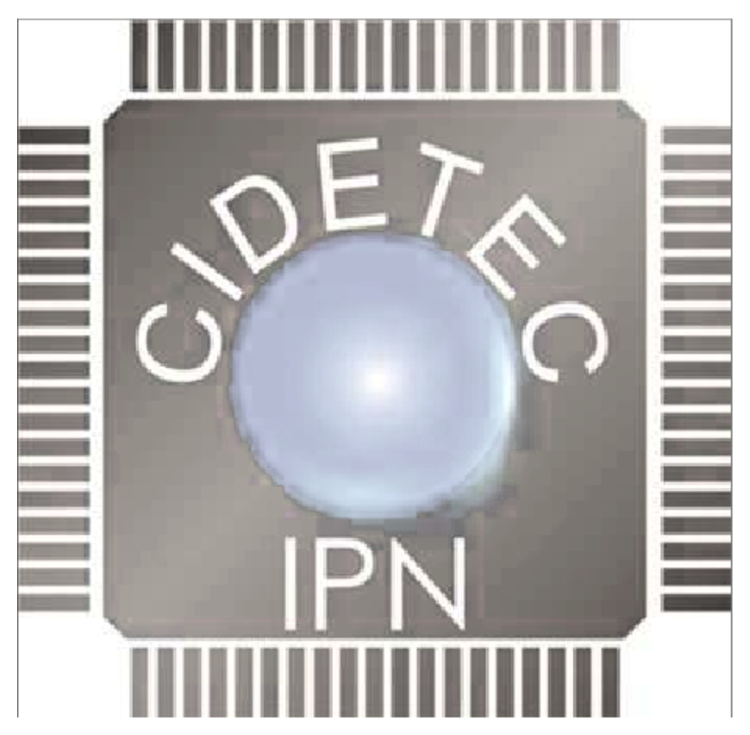
\includegraphics[width=.5cm]{Logos/logo_cidetec1.eps}
 \normalsize\insertframenumber} 

\title[Tesis]{\small\textbf{Sistema de aprendizaje no supervisado para la 
 detecci\'on y automatizaci\'on de tareas repetitivas en el entorno de una 
  computadora}}

\author[Gonz\'alez Tello]{
\textbf{\footnotesize Presenta:}\\
[0.1cm]{\footnotesize Ing.Ricardo Gonz\'alez Tello \\
[0.2cm] \footnotesize\textbf{Directores:} \\
[0.1cm] \footnotesize Dr. Jos\'e F\'elix S\'errano Talamantes \\
[0.1cm] \footnotesize Dr. Mauricio Olgu\'in Carbajal}
}

\date{\footnotesize México, Ciudad de México \hspace{2.5cm}
      \footnotesize Diciembre de 2018}

\renewcommand{\tablename}{Tabla}
\renewcommand{\figurename}{Figura}